%%%%%%%%%%%%%%%%%%%%%
%%% ANALISIS CORRELACIONAL
%%%%%%%%%%%%%%%%%%%%%%%%
\section{An�lisis correlacional}

El an�lisis de las variable de muestra que existe una relaci�n entre la satisfacci�n de la carrera y la elecci�n de carrera, esta correlaci�n  provee un indice de Pearson de  0.88.  Esto demuestra que existe una correlaci�n positiva entre ambas variables de inter�s\\

\begin{table}[H]
	\begin{center}
		\caption{Correlaci�n de Pearson entre satisfacci�n en la carrera y la elecci�n de la misma}
		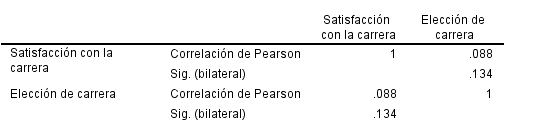
\includegraphics[scale=0.95]{ANA_CORRE_IMG1}
	\end{center}
\end{table}